\documentclass{ximera}

\ifdefined\HCode
  \newcommand{\alttext}[1]{\HCode{<span class="sr-only">#1</span>}}
\else
  \newcommand{\alttext}[1]{} % Fallback for PDF view
\fi

% MATH -----------------------------------------------------------
\newcommand{\nats}{\mathbb N}
\newcommand{\ints}{\mathbb Z}
\newcommand{\rats}{\mathbb Q}
\newcommand{\reals}{\mathbb R}
\newcommand{\complex}{\mathbb C}
\newcommand{\powerset}{\mathscr P}

%-------------------------------------------------------------

\pgfplotsset{compat=1.18}
\begin{document}
\begin{abstract}
 \end{abstract}

    \title{Class Discussion Activity 1}
    
    \maketitle

\section*{Exercises}

\begin{enumerate}[label=(\arabic*)]

\item Determine which first order differential equation has the following slope field.



\begin{figure}[h]
    \centering
\alttext{A direction field.}
\begin{tikzpicture}[scale=0.9,
    declare function = {f(\x) = \x*\x*\y;} % Define which function we're using
    ]
    \begin{axis}[
        zmax = 1,
        zmin = 0,
        xtick = {-1,-0.5,...,1},
        axis equal image = true, % Unit vectors for both axes have the same length
        view = {0}{90}
        ]
        \addplot3[% Arrows' first-half
            blue,
            -stealth,
            domain  = -1:1,
            samples = 20,
            quiver  = {
                u=1/(2*sqrt(1^2 + f(x)^2)),
                v=f(x)/(2*sqrt(1^2 + f(x)^2)),
                scale arrows=0.075,
                },
        ] (x,y,0);
        \addplot3[% Arrow's second-half
            blue,
            domain  = -1:1,
            samples = 20,
            quiver  = {
                u=-1/(2*sqrt(1^2 + f(x)^2)),
                v=-f(x)/(2*sqrt(1^2 + f(x)^2)),
                scale arrows=0.075,
                },
        ] (x,y,0);
    \end{axis}
\end{tikzpicture}
    \caption{A direction field (also known as a slope field)}
\end{figure}

 \begin{enumerate}[label=(\alph*)]
    \item $y^{\,\prime}=xy$
    \item $y^{\,\prime}=x^2y$ % ***
    \item $y^{\,\prime}=xy^2$
    \item $y^{\,\prime}=x^2y^2$
    \item $y^{\,\prime}=x/y$
    \item $y^{\,\prime}=y/x$
    \end{enumerate}

    \newpage

\item On which intervals is the function $y(x)=\dfrac{1}{1-\ln{(x)}}$ a solution to $xy'=y^2$?  Select all that apply.\\

%  y'=1/[x(1-ln(x))^2] ---> xy'=y^2


\begin{enumerate}
\item $(-\infty,\infty)$\\
\item $(-\infty,0)$\\
\item $(0,1)$\\ % ***
\item $(0,e)$\\  % ***
\item $(0,\infty)$\\
\item $(1,\infty)$\\
\item $(e,\infty)$\\ % ***
\end{enumerate}

% (c), (d) and (g) with option through (g)
    
\item Find a real value of the parameter $k$ such that $y=e^{kt}$ is a solution to $y^{\,\prime\prime}-y^{\,\prime}-12y=0$.\\

% -3 OR 4

\item Find a real value of the parameter $m$ such that $y=x^m$ is a solution to the differential equation $10x^2 y\,''+23xy\,'-3y=0$.\\

    % 0.2 OR -1.5

    % (5m-1)(2m+3)=10m^2+13m-3



\item    A 1st order differential equation $y'=f(t,y)$ with a so-called $``$initial condition" $y(t_0)=y_0$ is called an \underline{Initial Value Problem} (abbreviated $``$IVP").  An $``$IVP solution" must satisfy both the differential equation and the initial condition.  There is a unique solution $y(t)$ to the 1st order IVP $ty^{\,\prime}-y=-\dfrac{200}{t}$, $y(1)=101$ on the interval $(0,\infty)$.  Find $y(2026)$ to the nearest hundredth.\\

% mu=t^(-1).  So (mu y)' = -200 t^(-3) ---> mu y=100t^(-2)+C so y=100/t +ct.  101=100+c so c=1. 

% So y=100/t+ t

% y(2026)=100/2026+2026 \approx 2026.05


\item Determine the width of the widest open interval on which there is a solution to the IVP $y\,'+\dfrac{2xy}{x^2-1}=3$, $y(0)=1$.  If the answer is infinity, enter $-1$ in the quiz question. \\

% 2 since it is (-1,1).

% I.F.=x^2-1, so [(x^2-1)y]'=3x^2-3 ---> (x^2-1)y=x^3-3x+C ---> y=(x^3-3x-1)/(x^2-1).



\newpage


\item Suppose $y(x)$ satisfies the IVP $\displaystyle y'+\frac{2xy}{x^2+1}=3e^{x^3+3x}$, $y(0)=0$.  Determine $y(1)$.  Round to the nearest tenth.\\


% [(x^2+1)y]'=(3x^2+3)e^(x^3+3x)
% (x^2+1)y=e^(x^3+3x)+C
% y=[e^(x^3+3x)-1]/(x^2+1)

% y(1)=(e^4-1)/2\approx 26.8



\item  Any integral curve (or part of an integral curve) of a differential equation is made up of solution curves to that differential equation.  What is the minimum number of solution curves needed to form the part of an integral curve to $y\,'=\dfrac{x^2}{1-y^2}$ depicted below?

    % 3

\begin{figure}[h]
\centering
   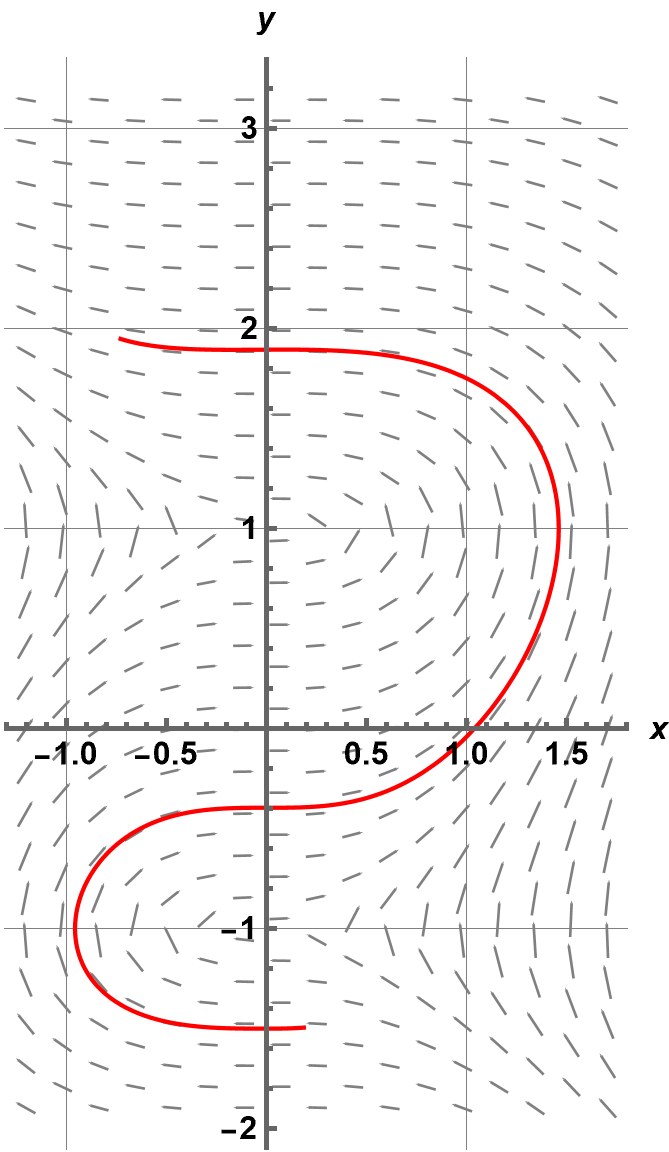
\includegraphics[scale=0.7,alt={An integral curve in a direction field.}]{IntegralCurveFromThreeSolutionCurves.png}
   \caption{An integral curve in a direction field}
\end{figure}



\newpage


\item  On which of the following open intervals is it guaranteed that there is \textbf{NO solution} to the IVP $(x+1)y^{\,\prime}+y=1$, $y(0)=2$?  Select all that apply.

% y = 1 + 1/(x+1)
% y' = -(y-1)/(x+1)

 \begin{enumerate}[label=(\alph*)]
    \item $(-\infty,\infty)$% ***
    \item $(-1,1)$
    \item $(-1,\infty)$
    \item $(-\infty,1)$ % ***
    \item $(-2,1)$  % ***
    \item $(-2,2)$  % ***
    \item $(-2,-1)$ % ***
    \item $(-1,2)$
    \end{enumerate}

% a,d,e,f,g ... h

\item Suppose an epidemic spreading through a certain population is modeled by the differential equation $y^{\,\prime}(t)=ay(t)-b[y(t)]^2$ where $a,b$ are positive constants and $y(t)$ is the number of individuals who have the disease at time $t$ days.  Below is a direction field for such a model.  Suppose we are given that $a=0.75$ and $\displaystyle \lim_{t\rightarrow\infty} y(t)=6,000$ for any non-trivial solution $y(t)$.  Determine $b$. Round to the nearest ten-thousandth.


\begin{figure}[h]
\centering
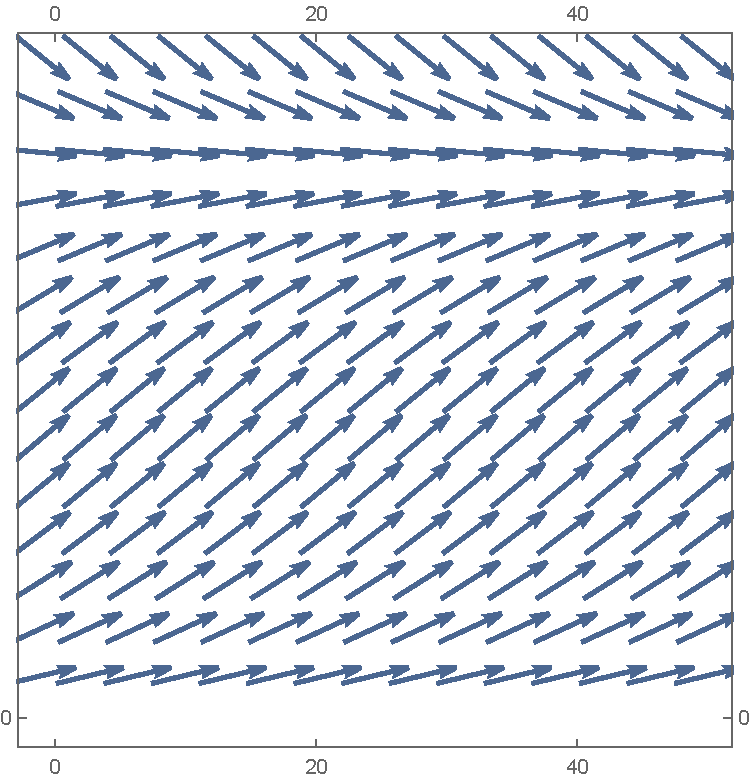
\includegraphics[scale= 0.7,alt={A direction field.}]{UnkLogisticAct1.pdf}
\caption{Another direction field}
\end{figure}

% 0.75/6000=b \approx 0.0001


\end{enumerate}



\end{document}